\chapter{Thermal-SZ Weak Lensing Cross Correlation}
\label{cross_correlation}
\section{Calculation from Data}
\label{tszcross}
Once the tSZ maps are found using the above method, we cross-correlate the the tangential
shear component using the Weak-Lensing datasets available.
We compute the cross correlation using
the k-D trees algorithm. k-D trees perform efficiently in nearest neighbour searches and help
speedup calculating the correlation functions significantly. We use the \texttt{treecorr} library
for this \cite{treecorr}. We perform the cross correlation
using the  Red Cluster Sequence Lensing Survey (RCSLens) dataset \cite{rcslens}
and the Planck tSZ skymaps \cite{plancksz}, initially, to verify our cross correlations by
comparing the results with \cite{tszrcscross}.
We repeat the same with the Kilo Degree Survey (KiDS) dataset \cite{kidsdr4} and
our own tSZ skymaps.

Following this, we will compare with different theoretical predictions will help us
constrain the cosmology and baryon models. Especially, We are interested in looking at
non-gravitational feedback.

For $y-\gamma_T$, we compute the two point correlation function as, 
\begin{align}
  \begin{split}
    \xi^{y - \gamma_T}(\theta) = \frac{\sum\limits_{ij} y^i e^{ij}_t w^j \Delta_{ij}(\theta)}{\sum\limits_{ij} w^j \Delta_{ij}(\theta)}
  \end{split}
\end{align}
where, $y^i$ is the y-value from the tSZ maps in pixel i. And $e^{ij}$ is the tangential ellipticity of the galaxy j in the catalogue with
respect to pixel i. The tangential ellipticity is corrected for both multiplicative and additive bias. $\Delta_{ij}(\theta)$ imposes our binning scheme.
It is one if the angular seperation between i and j is $\theta$ and zero otherwise.

\section{k-D Trees Algorithm}
k-D trees is a space partitioning algorithm which stores the coordinates in a tree data structure,
the algorithm constructs the tree based on the proximity of the points without explicitly computing the distances between
the points.
\begin{figure}[htbp]
  \centering
  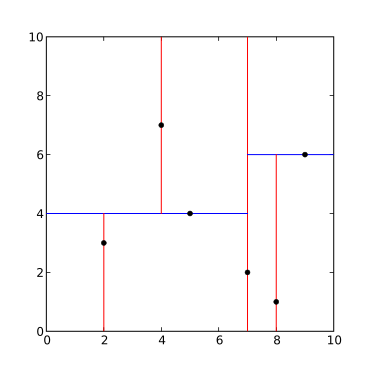
\includegraphics[width=0.3\linewidth]{kdtree_2d.png}
  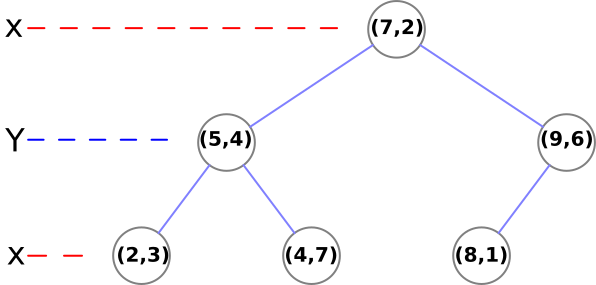
\includegraphics[width=0.3\linewidth]{tree_2d.png}
  \caption{Example k-D Trees partitioning and data structure}
\end{figure}
Finding the nearest neighbours then becomes merely the act of traversing the trees. This immensely speeds
up the computation of correlation functions.

\section{Systematic Tests}
In order to test for systematics in the data, We perform 2 systematic tests.
\begin{itemize}
\item We calculate $\langle y \gamma_x \rangle$
\item We randomise the catalogue and find the correlation once again.
\end{itemize}
in the absence of systematic errors, in our calculation. Both of these tests should give us values close to zero.



\section{Comparison with Theory}
\label{theory}
We like to compare our observations with theoretical predicitions based on Halo models, closely
following the method developed by 
\cite{halotheoryma}. Currently we are concentrating on computing the real space cross correlation
$ \xi = \langle \gamma_T - y \rangle$ , By using
\begin{equation}
  \label{realcrosstheory}
  \xi^{y - \gamma_T} (\theta) = \int \frac{d^2 \vec{l}}{2\pi^2 } C_l^{y-k} \cos(2(\phi - \psi)) \exp(i \theta \cos(\phi - \psi))
\end{equation}
Where, $\phi$ is the Polar angle with respect to the coordinate system and $\psi$ is the angle
between $\vec{l}$ and the coordinate.

In order to compute the $y - k$ cross correlation power spectra found in Equation
\ref{realcrosstheory}, we use the 1-halo term as defined in \cite{haloreview}.
\begin{equation}
  C_l^{y-k,1h} = \int\limits_0^{z_{max}} dz \frac{dV}{dz d\Omega} \int\limits_{M_{min}}^{M_{max}} dM \frac{dn}{dM} y_l (M, z) k_l (M,z)
\end{equation}
For the halo mass function, We use the form suggested by Sheth and Tormen \cite{massfunctionsheth}
For the convergence profile in fourier space, We use
\begin{equation}
  k_l = \frac{W^k(z)}{\xi^2(z)} \frac{1}{\rho_m} 4 \pi \int\limits_0 ^{r_{vir}} dr r^2 \frac{\sin(lr/\xi)}{lr/\xi} \rho(r;M,z)
\end{equation}
   \\
And for the fourier transform of the projected gas pressure.
\begin{equation}
    y_l = \frac{4 \pi r_s}{l^2_s} \frac{\sigma_T}{m_e c^2} \int dx x^2  \frac{\sin(lx/\xi)}{lx/\xi} P_e(x;M,z)
\end{equation}
\\
For electron pressure, We use the \emph{universal pressure profile} and the NFW model. 
We plan to use the best fit parameters for the Pressure profile from the Planck Collaboration
and then compare the halo model predictions from both the Planck and WMAP-7yr cosmologies. To look
for any non-gravitational feedback, we plan to use the method developed by \cite{subhapaper},
applied to tSZ $C_l$s.


%%% Local Variables:
%%% mode: latex
%%% TeX-master: "thesis"
%%% End:
